\section{Dataset}

Multiple iterations of the recording process were run to find the best possible setup, which reduces the light interference as much as possible and which offers the best results with the resources at hand. The camera setup that is used by SilverFit was reproduced. At SilverFit the camera is mounted at $175cm$ above the floor. The camera that is used has an accelerometer which was used to adjust the camera angle relative to the ground. The camera is angled downward at a $70^\circ$ angle. 

\subsection{Problem Sets}
\label{sec:problem_set}

Different problem sets are used to create different versions of the model. The problem sets are defined by the number of objects that are considered and are defined as erroneous. There are four different problem sets. The first problem set is the \textit{Joint} problem set. In this problem set, each joint is considered as a single object. The second problem set,  the \textit{Limb} problem set, is to consider each limb, i.e. the individual arms, legs, torso, and head. The third problem set is the \textit{Half Body} problem set. In this problem set the upper and the lower body are the areas that are considered. Finally, only the whole body is considered in the \textit{Full Body} problem set.

To determine the threshold at which each area is considered faulty, the number of errors by area was calculated and the 50th percentile was measured. The goal of this is to result in a more balanced dataset. In Figure \ref{fig:dist_jt_epp} the distribution of joints with errors can be seen. The red line shows the 50th percentile of the distribution, i.e. $50\%$ of the frames contains more errors than the position that is marked. For example, in Figure \ref{fig:dist_jt_epp}, the 50th percentile is at 2 Joints with errors, i.e. if the frame has more than two joints which have an error the Full Body is considered as faulty.

\begin{figure}
  \centering
  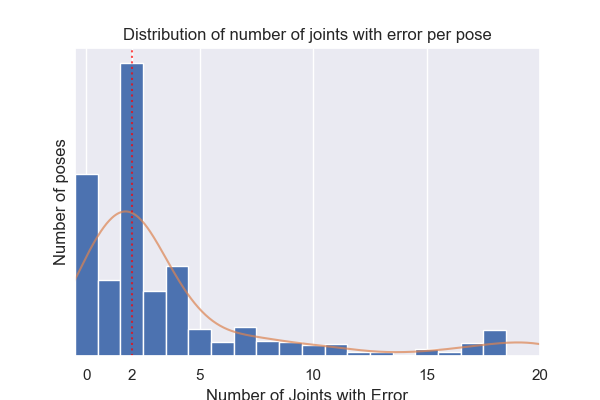
\includegraphics[width=0.8\textwidth]{figures/Data/joint_errors_per_pose/distribution_of_joint_errors_per_pose.png}
  \caption[Number of Joints with error]{The distribution of the number of joints with errors in each frame.}
  \label{fig:dist_jt_epp}
\end{figure}

Similarly, Figure \ref{fig:dist_bh_epp} shows the distribution of joints with errors for the Half Body problem set. The upper half is considered erroneous if one joint in the upper body is faulty. If more than two joints are labelled as incorrect in the lower half of the body then the lower body is labelled likewise.

\begin{figure}
  \centering
  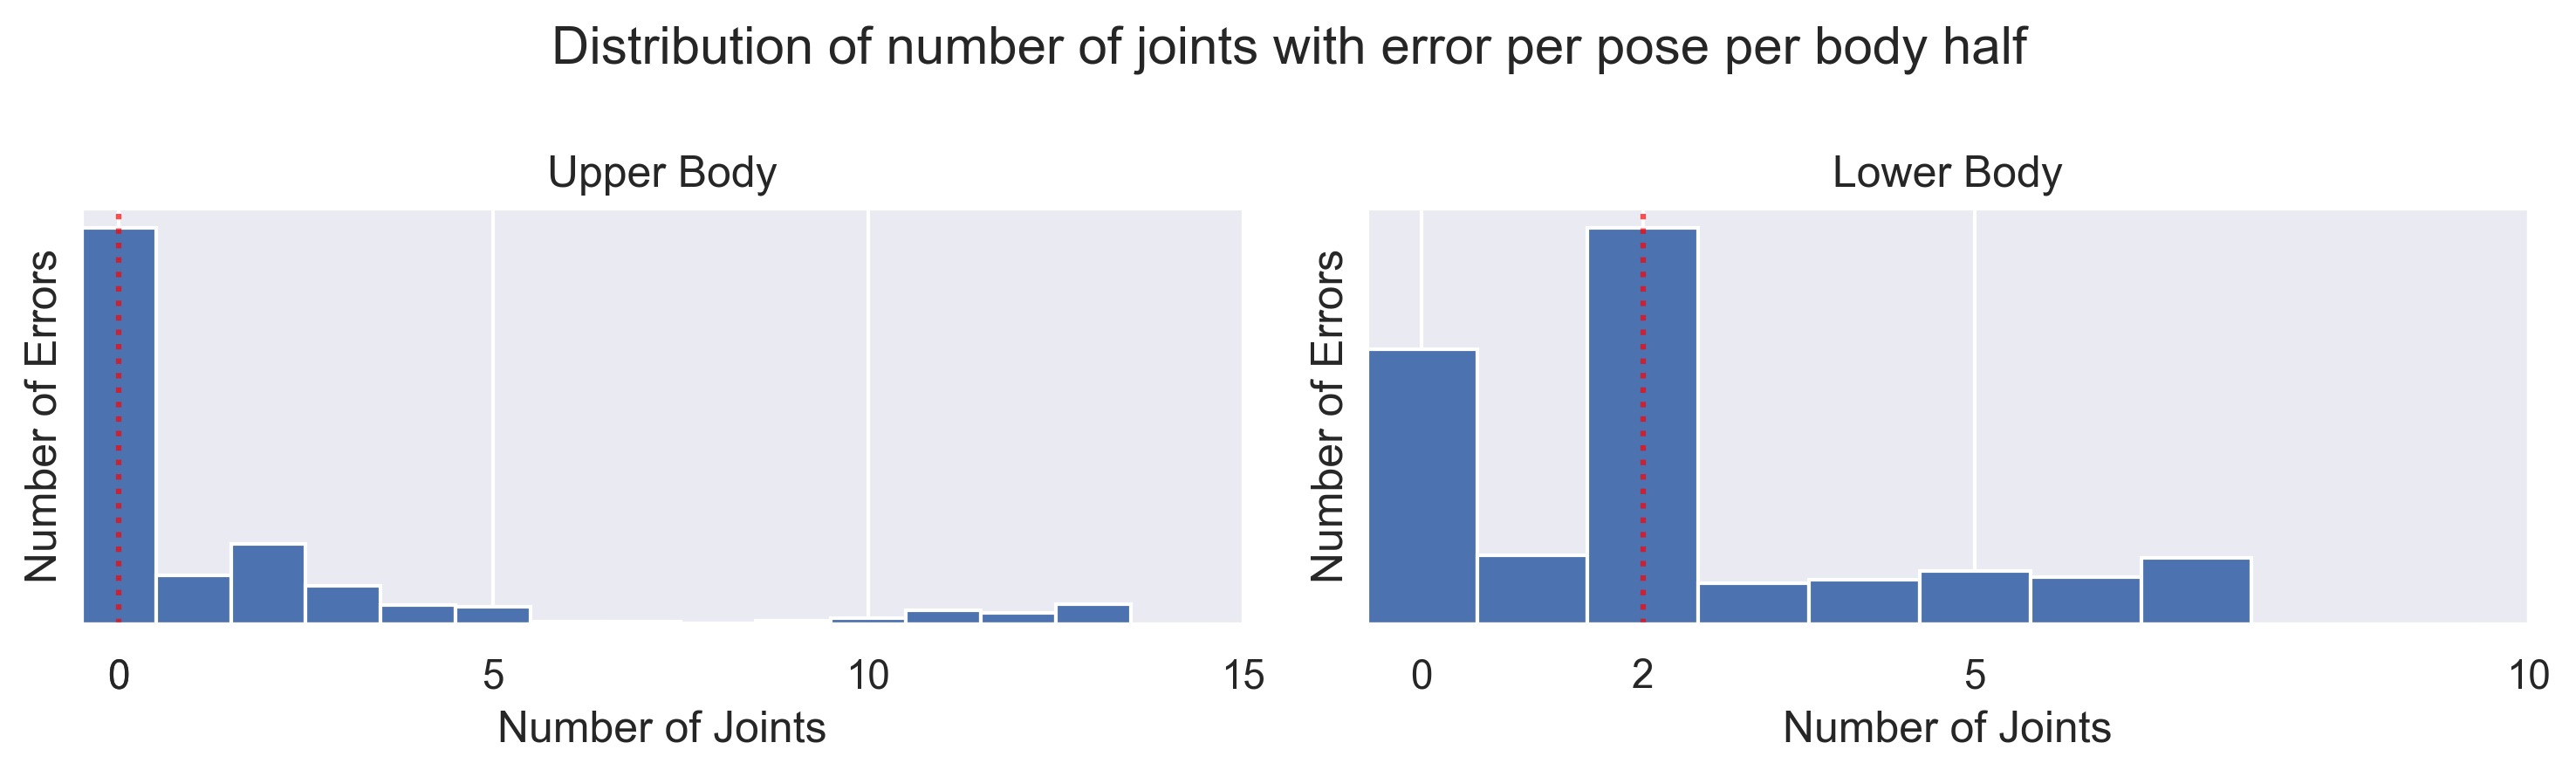
\includegraphics[width=0.8\textwidth]{figures/Data/joint_errors_per_pose/distribution_of_joint_errors_per_pose_per_body_half.png}
  \caption[Number of Joints with error per body half]{The distribution of the number of joints with errors in each frame per body half.}
  \label{fig:dist_bh_epp}
\end{figure}

Finally, the individual limbs are investigated. Figure \ref{fig:dist_lb_epp}, shows the distribution of joints with errors for each of the limbs. All limbs except for the legs are considered faulty if one or more joints in that limb are faulty. The legs are considered erroneous if there is more than one faulty joint.

\begin{figure}
  \centering
  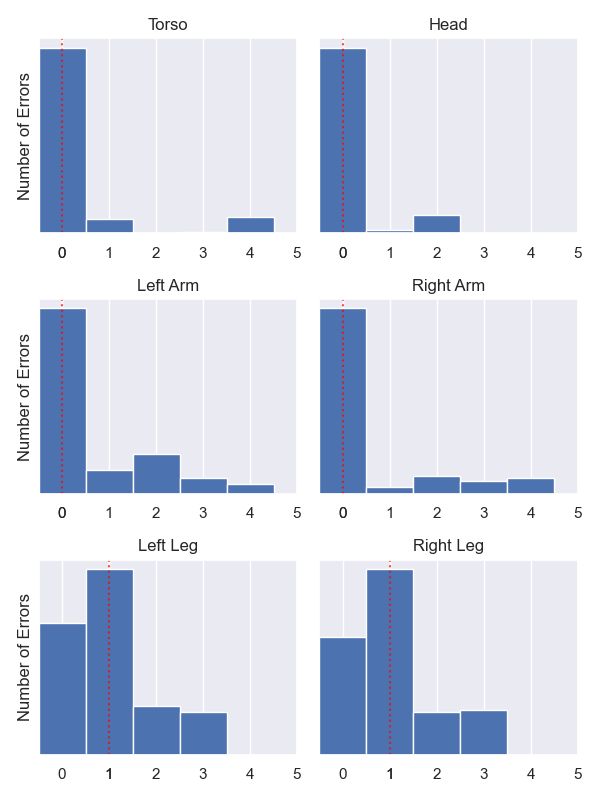
\includegraphics[width=0.6\textwidth]{figures/Data/joint_errors_per_pose/distribution_of_joint_errors_per_pose_per_body_part.png}
  \caption[Number of Joints with error per limb]{The distribution of the number of joints with errors in each frame per limb.}
  \label{fig:dist_lb_epp}
\end{figure}

\subsection{Distribution of Errors}
% in one view a global statistic and in the appendix

An important aspect of the dataset is the structure and distribution of data and their labels. In total, all 13 exercises mentioned in Section \ref{sec:exercises} were recorded twice. Each recording session consists of exactly 300 frames.

When multiple persons are detected one person might be incorrectly detected in the background. While analysing the data the person that is not labelled as faulty is selected whenever possible. If a person is labelled as faulty each joint is marked as in an unrealistic position.

An important factor in how well a model can be trained on data is the balance of the dataset. In this case, the dataset is balanced by the error labels. 

\subsubsection{Full Body Error Distribution}

In Figure \ref{fig:fb_pie} the error distribution of the Full body problem set can be seen. It can be observed that the distribution of errors is reasonably equal with a difference of $10\%$. 

\begin{figure}
  \centering
  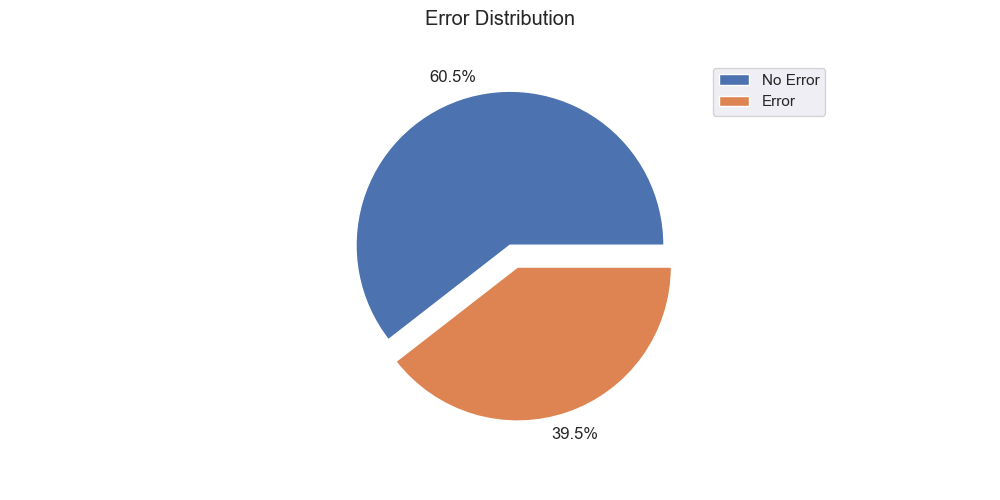
\includegraphics[width=0.8\textwidth]{figures/Data/dist_full_body/Error_Distribution_by_Body_Half.png}
  \caption[Error Distribution of the Full Body]{The distribution of Errors of the full body problem set.}
  \label{fig:fb_pie}
\end{figure}

Figure \ref{fig:fb_diff_dist} gives an overview of the error distribution by the difficulty of the exercise. The figure indicates that the difficulty of the exercise directly influences the percentage of errors that occur.

\begin{figure}
  \centering
  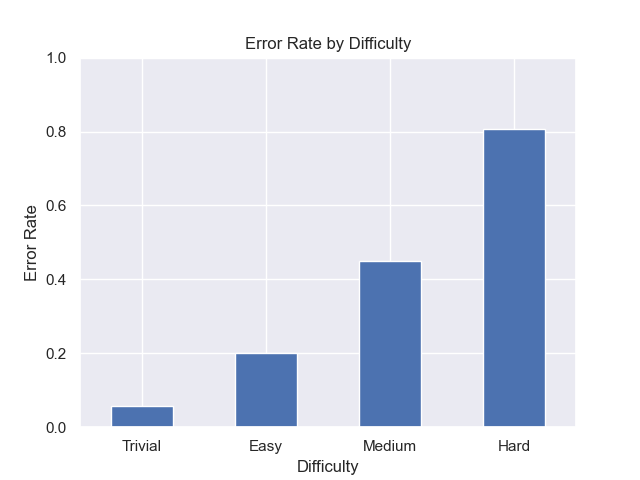
\includegraphics[width=0.8\textwidth]{figures/Data/dist_full_body/Error_Rate_by_Difficulty.png}
  \caption[Error Distribution of the Full Body by difficulty]{The distribution of Errors of the full body problem set by difficulty.}
  \label{fig:fb_diff_dist}
\end{figure}


\subsubsection{Half Body Error Distribution}

Figure \ref{fig:hb_pie} shows a discrepancy between the error distribution of the lower body ($65.4\%$ Errors) and the upper body ($32.4\%$ Errors). The upper body is generally more stable and less error-prone than the lower body.

\begin{figure}
  \centering
  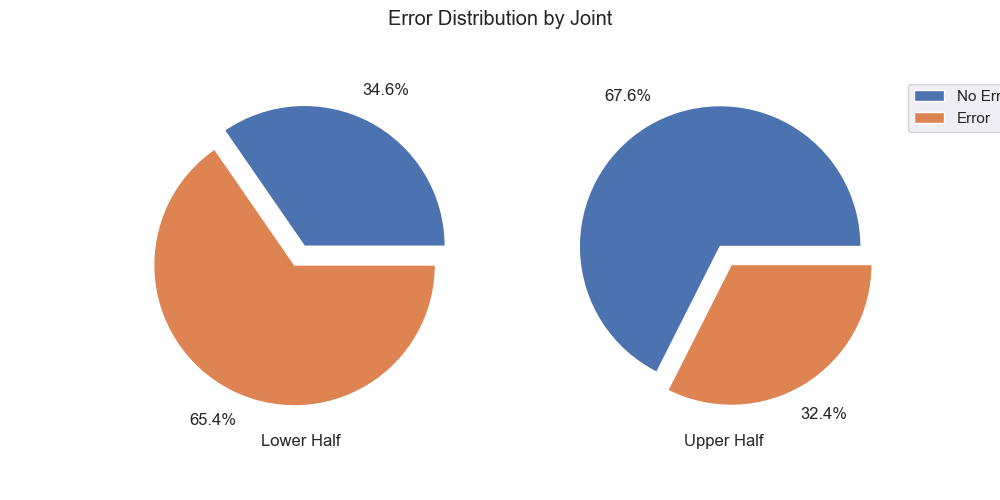
\includegraphics[width=0.8\textwidth]{figures/Data/dist_half_body/Error_Distribution_by_Joint.png}
  \caption[Error Distribution by Body Half]{The distribution of Errors of the half body problem set.}
  \label{fig:hb_pie}
\end{figure}

The distribution of errors by difficulty can be seen in Figure \ref{fig:hb_diff_dist}. Easy exercises seem to be less error-prone when grouping the joints into body halves. This might be caused by the error threshold that was set before.

\begin{figure}
  \centering
  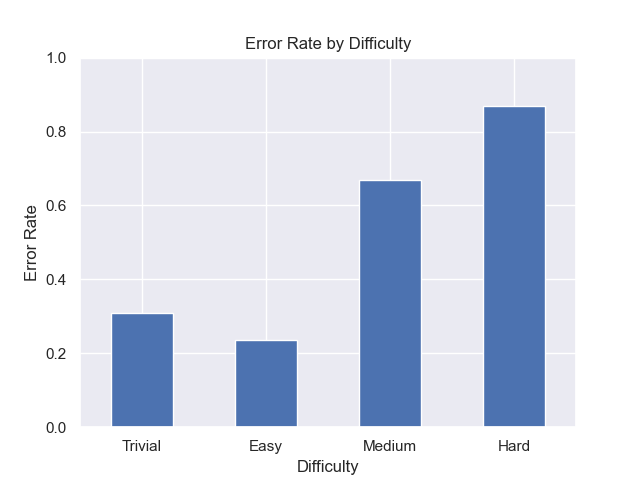
\includegraphics[width=0.8\textwidth]{figures/Data/dist_half_body/Error_Rate_by_Difficulty.png}
  \caption[Error Distribution of the Half Body by difficulty]{The distribution of Errors of the half body problem set by difficulty.}
  \label{fig:hb_diff_dist}
\end{figure}

\subsubsection{Limb Error Distribution}

The error distribution of each limb is shown in Figure \ref{fig:lb_pie}. It can be observed that the errors of the limbs are individually very unbalanced. The left arm is the most error-prone limb with $24.1\%$ of the joints being faulty. The torso is the least error-prone limb with $10.3\%$ of the joints being faulty. This again underlines the assumption that the upper body is more stable than the lower body.

\begin{figure}
  \centering
  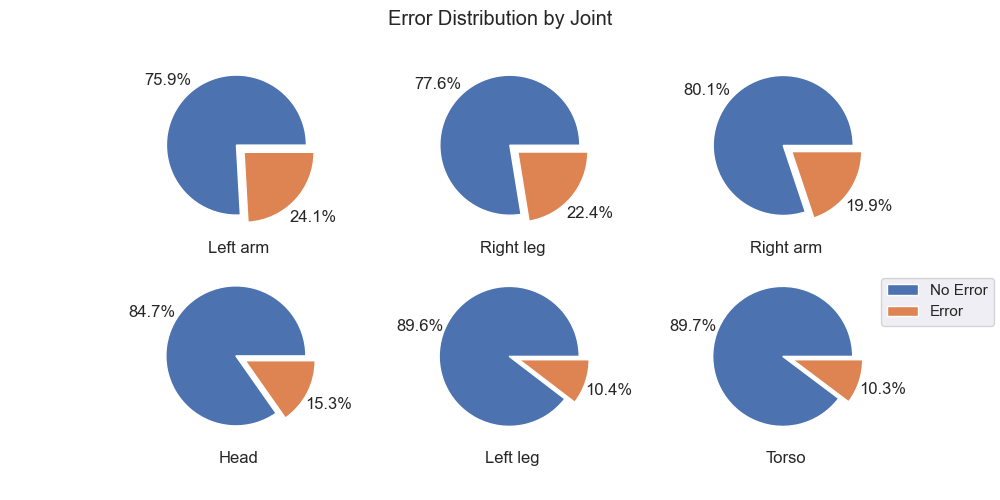
\includegraphics[width=0.8\textwidth]{figures/Data/dist_limbs/Error_Distribution_by_Joint.png}
  \caption[Error Distribution by Limb]{The distribution of Errors of the limb problem set.}
  \label{fig:lb_pie}
\end{figure}

The distribution of errors by difficulty can be seen in Figure \ref{fig:lb_diff_dist}. A less distinct distribution of errors can be seen when grouping the joints into limbs. Only a very small amount of errors occur during trivial exercises. This might be caused by the error threshold that was set before. The majority of errors occurring during trivial exercises are caused by a single faulty joint in the ankle. In Figure \ref{fig:dist_lb_epp} it is shown that the legs have an error threshold of two faulty joints. This means that the legs are considered faulty if there are more than two faulty joints. The ankle is the only joint that is faulty in trivial exercises. This means that the legs are not considered faulty.

\begin{figure}
  \centering
  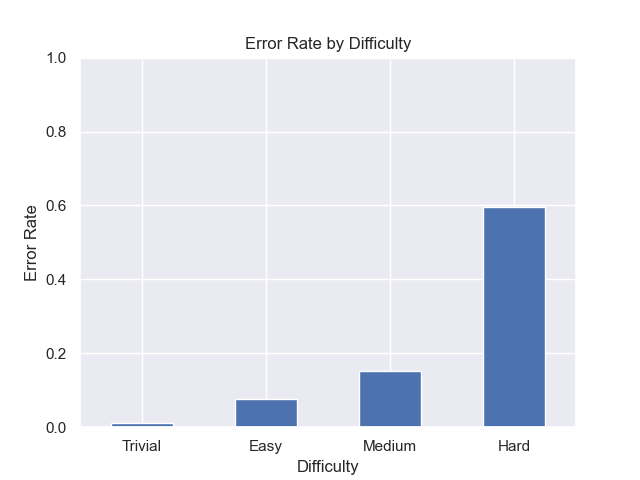
\includegraphics[width=0.8\textwidth]{figures/Data/dist_limbs/Error_Rate_by_Difficulty.png}
  \caption[Error Distribution of the limbs by difficulty]{The distribution of Errors of the half-body problem set by difficulty.}
  \label{fig:lb_diff_dist}
\end{figure}

\subsubsection{Joint Error Distribution}

Figure \ref{fig:jt_pie} shows that the major part of the errors that occur are Errors with the label 2, i.e. the joint is detected in the wrong place. The second most common error is label 1, i.e. the joint is not detected at all. The least common error is label 3, i.e. the joint is detected in the approximate position of where another joint should be.

\begin{figure}
  \centering
  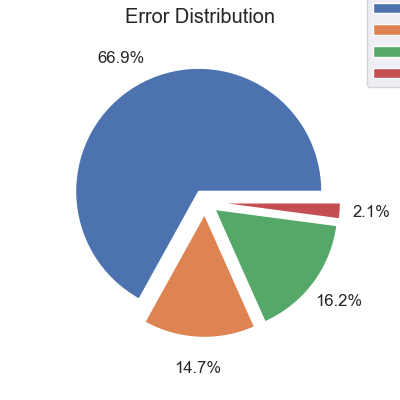
\includegraphics[width=0.4\textwidth]{figures/Data/dist_joints/Error_Distribution.png}
  \caption[Error Distribution for each error class]{The distribution of each error class.}
  \label{fig:jt_pie}
\end{figure}

In medium exercises, the majority of errors that occur, occur due to missing joints, rather than joints which are in the wrong position. This is shown in Figure \ref{fig:jt_pie_diff}.

\begin{figure}
  \centering
  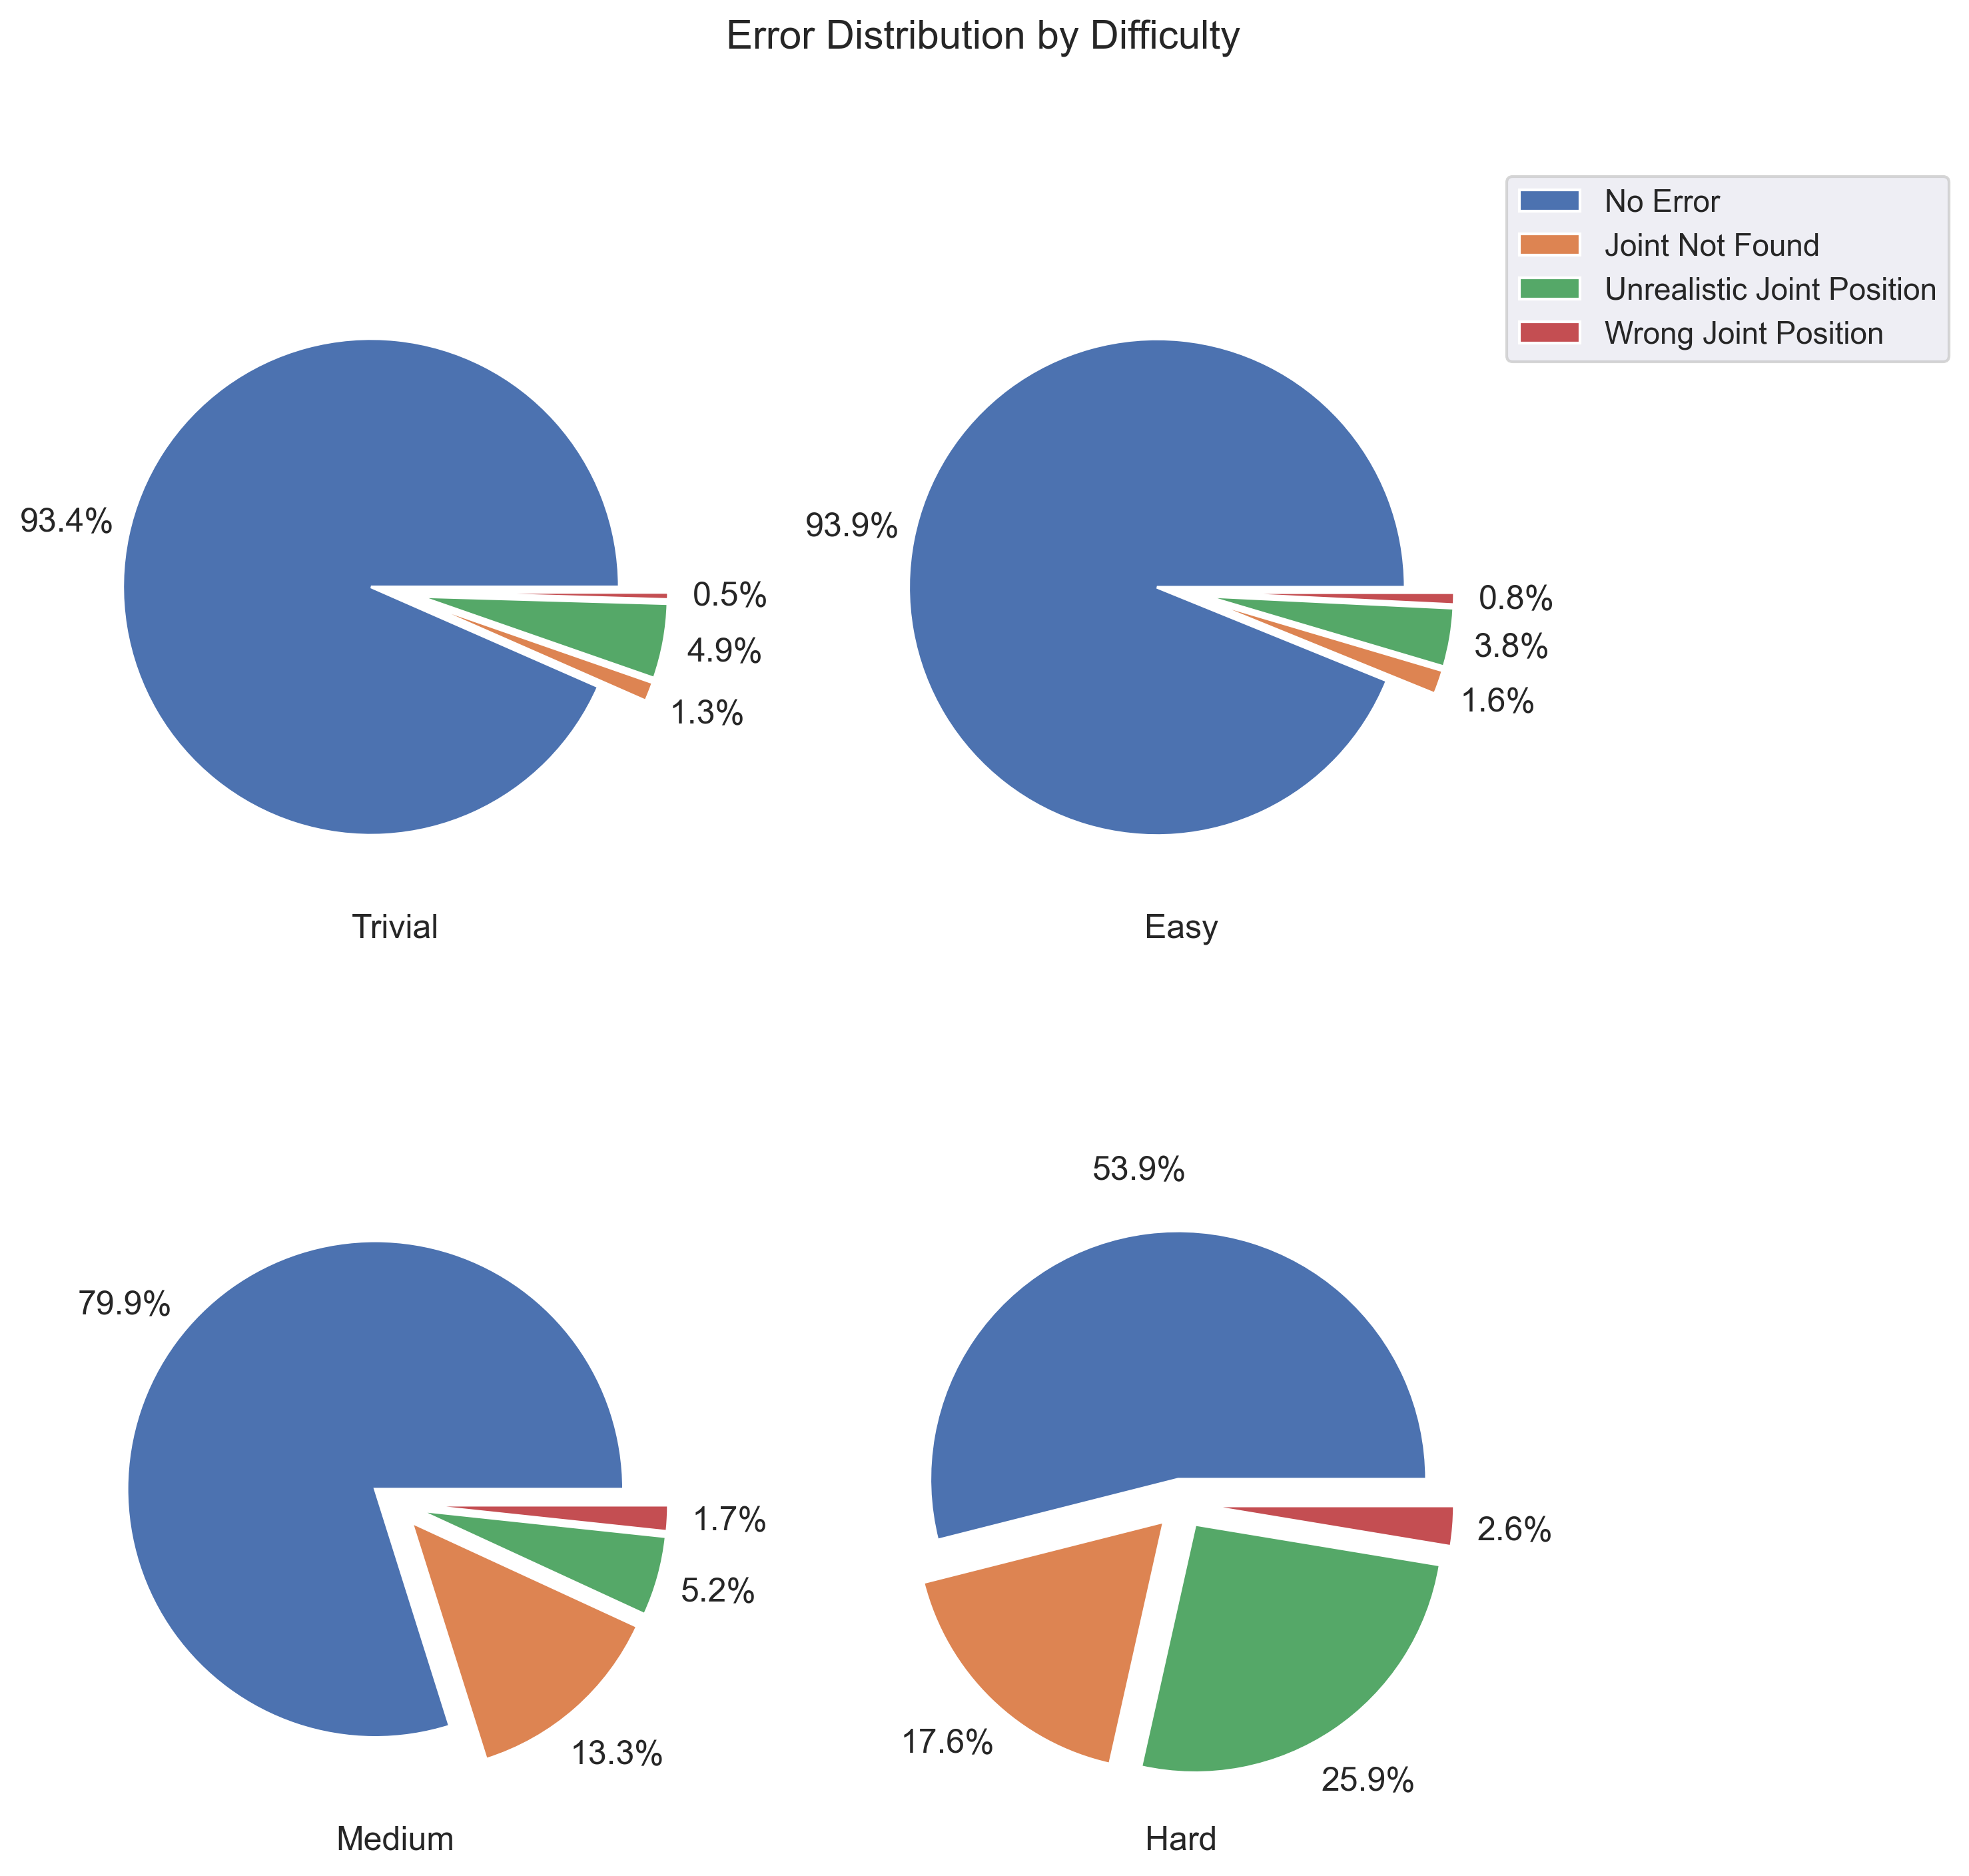
\includegraphics[width=0.8\textwidth]{figures/Data/dist_joints/Error_Distribution_by_Difficulty.png}
  \caption[Error Distribution for each error class by difficulty]{The distribution of each error class grouped by difficulty.}
  \label{fig:jt_pie_diff}
\end{figure}

A clear distinction between error-prone and stable joints can be seen in Figure \ref{fig:jt_pie_joint}. While in the majority of cases ($72.3\%$) the right ankle is faulty only $4.9\%$ of the left shoulder is faulty. Furthermore, the left and right ankles have a significant number of missing joints, contrary to the other joints, which have a more balanced distribution of error classes. This might be caused by occlusion or a cutoff from the image or a confidence which is too low and therefore discarded by Nuitrack.

\begin{figure}
  \centering
  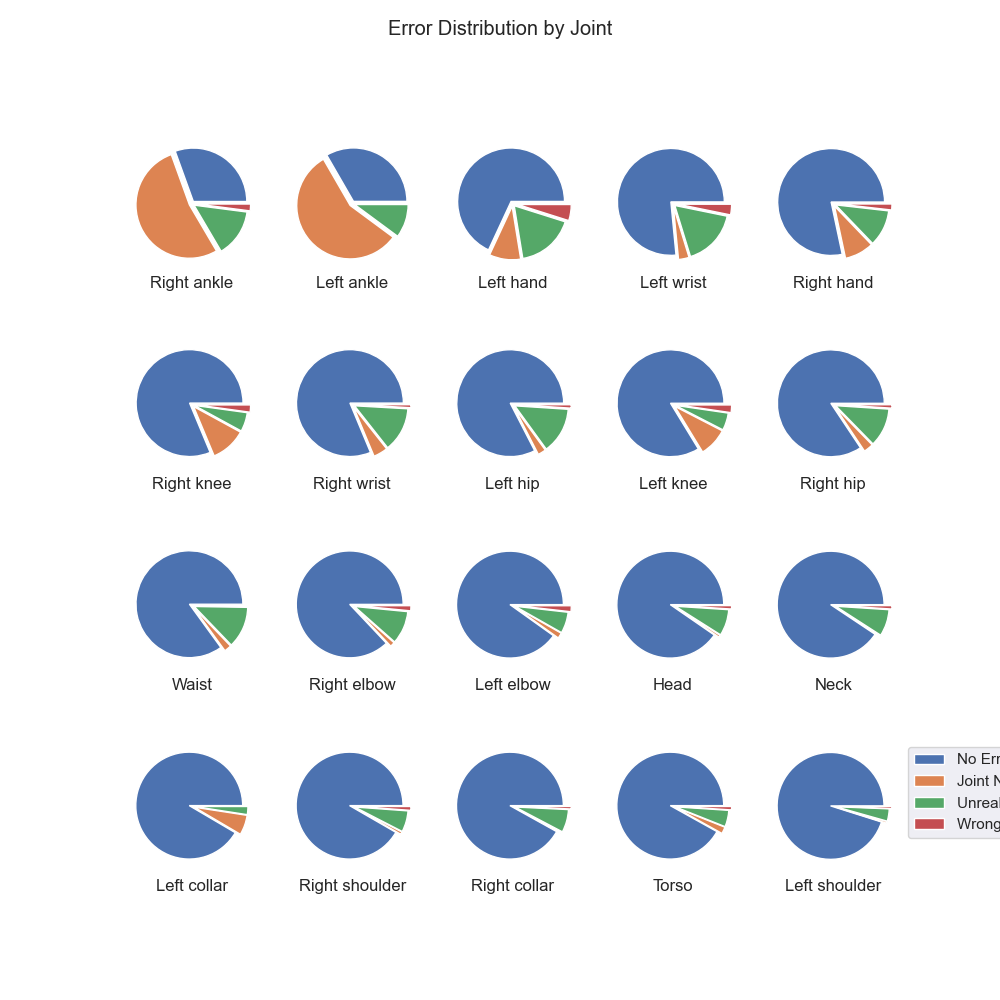
\includegraphics[width=0.8\textwidth]{figures/Data/dist_joints/Error_Distribution_by_Joint.png}
  \caption[Error Distribution for each error class by joint]{The distribution of each error class grouped by joint.}
  \label{fig:jt_pie_joint}
\end{figure}


\begin{figure}
  \centering
  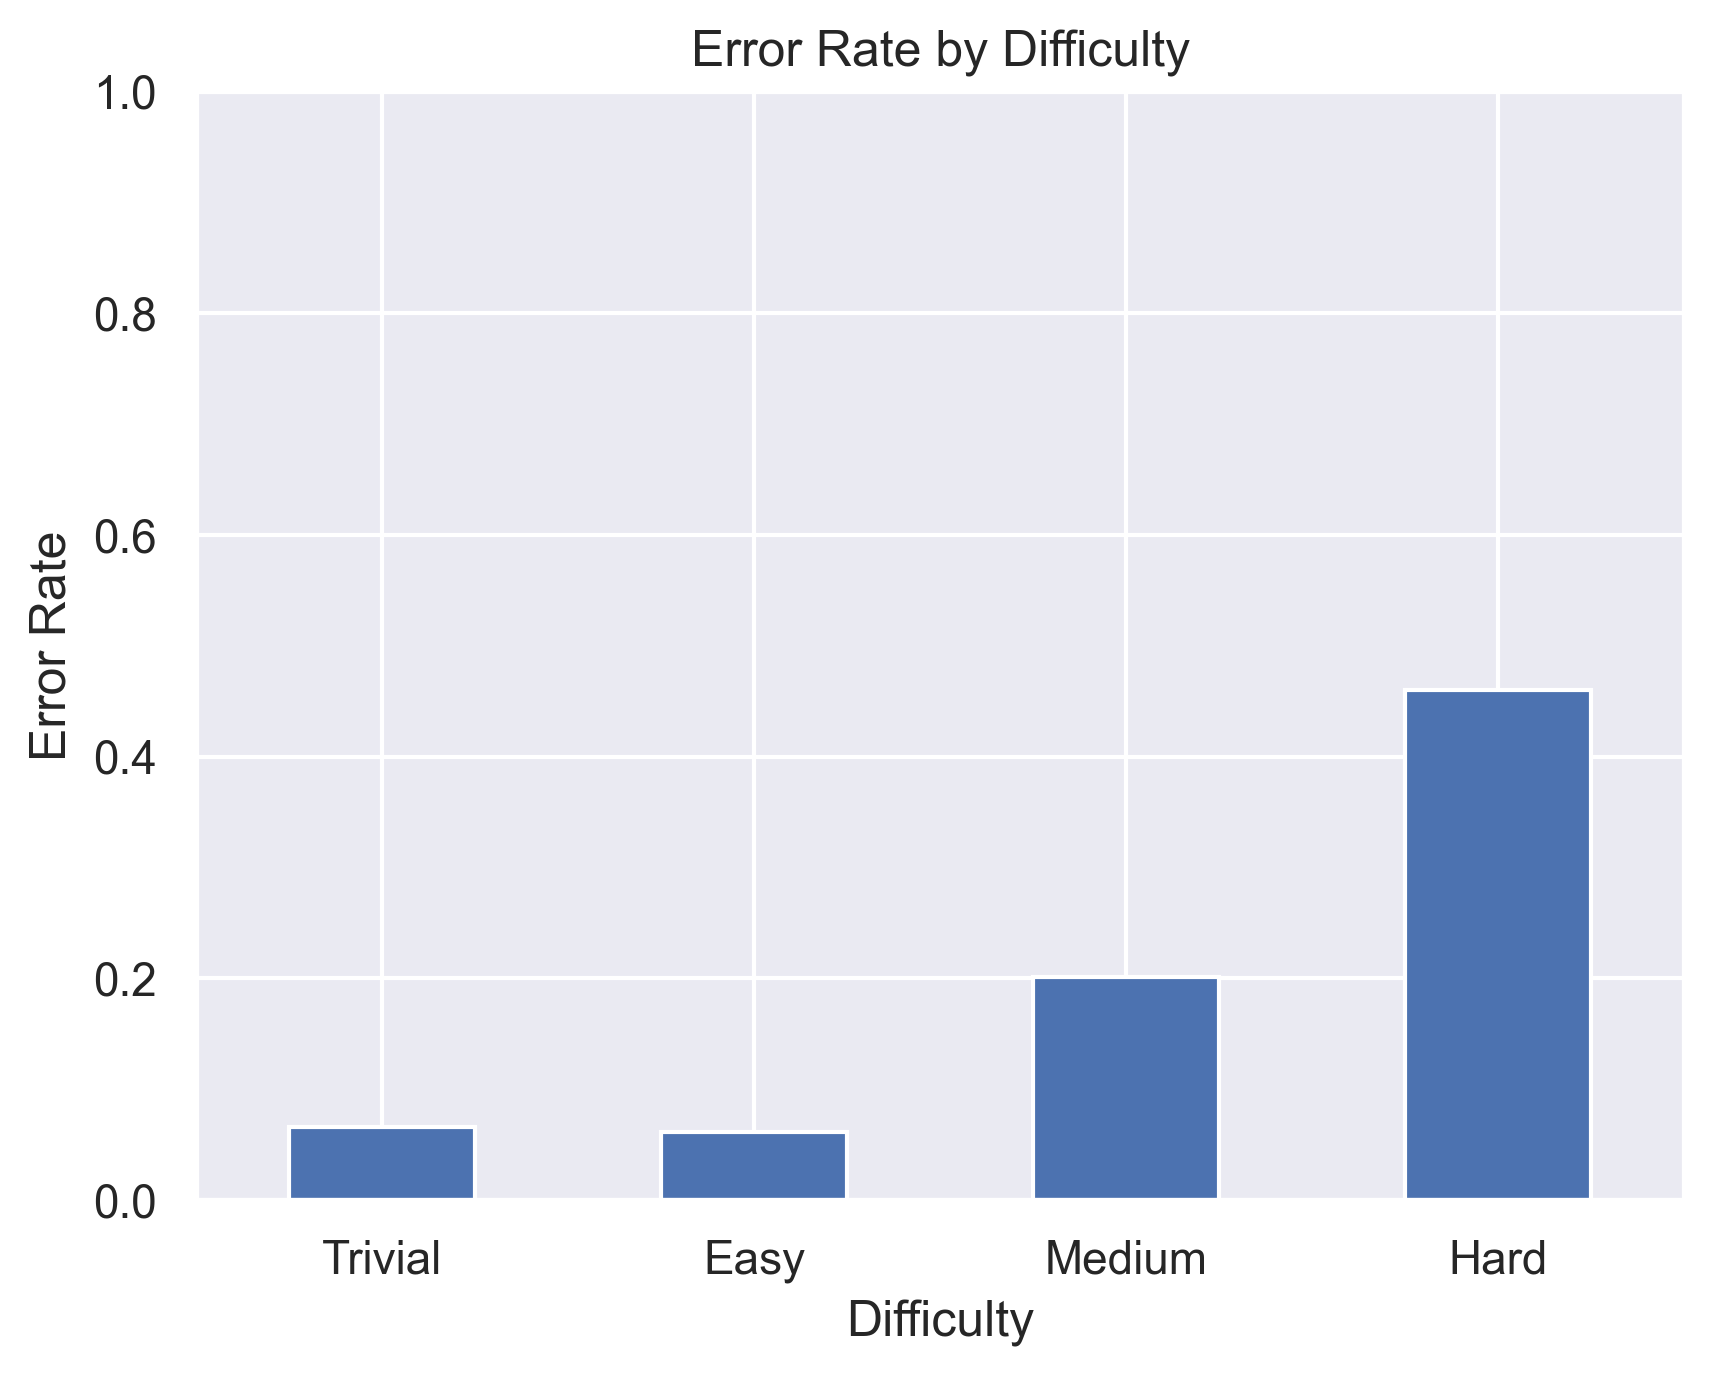
\includegraphics[width=0.8\textwidth]{figures/Data/dist_joints/Error_Rate_by_Difficulty.png}
  \caption[Error Distribution of the joints by difficulty]{The distribution of Errors of the joint problem set by difficulty.}
  \label{fig:jt_diff_dist}
\end{figure}

